\section{Aritmética}

\subsection{Operaciones con enteros}

\begin{questions}
    \question Resuelva las siguientes sumas mentalmente:
    \begin{multicols}{3}
    \begin{parts}
        \part $4 + 7 = $
        \part $5 + 9 = $
        \part $1 + 7 = $
        \part $13 + 8 = $
        \part $3 + 6 =$
        \part $16 + 6 =$
        \part $7 + 89=$
        \part $15 + 4 =$
        \part $2 + 149=$
        \part $5 + 18=$
        \part $6 + 72=$
        \part $54 + 9 =$
        \part $14 + 6 =$
        \part $35 + 97=$
        \part $92 + 8 =$
        \part $8 + 37=$
        \part $15 + 16=$
        \part $5 + 43=$
        \part $12 + 34 =$
        \part $13 + 17=$
        \part $7 + 43=$
        \part $28 + 7 =$
        \part $15 + 90 =$
        \part $9 + 43=$
        \part $6 + 104=$
        \part $8 + 14=$
        \part $8 + 82=$
        \part $9 + 12=$
        \part $7 + 67=$
        \part $9 + 23=$
        \part $2 + 926=$
        \part $12 + 35=$
        \part $213 + 77 =$
        \part $2 + 247=$
        \part $120 + 19=$
        \part $34 + 6=$
        \part $6 + 39=$
    \end{parts}
    \end{multicols}

    % \begin{EnvUplevel}
    % Como en todo cálculo mental, queremos simplificar primero las operaciones. Sumar es más fácil que restar, por ejemplo si tengo $62-35$, una forma es preguntarse ¿cómo llego del 35 al 62? Primero sumo 5 para llegar al 40, luego sumo otros 20 para llegar al 60 (llevo 25) y luego otros 2. Por tanto, 27.
    
    % Otra opción es ir quitando poquitos al grande, por ejemplo si tengo $329-92$, le puedo primero quitar 20 al grande, quedando 309, y me faltan otros 72 por quitar $309-72$. Puedo quitar 2, quedando $307-70$ y ahora sí usamos el otro, de 70 a 100 hay 30, luego del 100 al 300 hay 200, llevo 230, y los 7 que quedan, 237.  

    % En las siguientes respuestas intentamos desglosar las operaciones. Cuando hacemos algo como $56-48=(50-48)+(56-50)$, lo que queremos decir es: del 48 al 50 ¿cuánto hay? y luego, del 50 al 56, y sumamos estas longitudes intermedias. Cuando pasamos de algo como $398 - 204$ a algo como $198-4$, vemos que hicimos una resta parcial, ``cancelamos una parte, 200, de la deuda, pero todavía faltan 4 de pagar.''

    % Otro truco usual, cuando tenemos que restar una cantidad muy cercana a ser ``redonda'' - o sea, que termine en 0 -, como en $765-198$, podemos ``pagar un poco más y qué nos den vuelto'', en este ejemplo, pagamos 200, entonces nos quedan 565, pero nos dan de vuelto 2, o sea que terminamos con 567. Esto en las siguientes soluciones lo escribimos como $765-198=765-200+2=565+2=567$.
    % \end{EnvUplevel}
    
    \question Resuelva las siguientes restas mentalmente
    \begin{multicols}{3}
    \begin{parts}
        \part $9 -2 =$
        \part $14 - 4 =$
        \part $8 - 5 =$
        \part $7 - 6 =$
        \part $13 - 6 =$
        \part $22 - 4 =$
        \part $67 - 5 =$
        \part $31 - 8 =$
        \part $56  - 32 =$
        \part $87 - 15 =$
        \part $100 - 19 =$
        \part $35 - 29 =$
        \part $39 - 24 =$
        \part $97 - 40=$
        \part $405 - 29 =$
        \part $56 - 39 =$
        \part $35 - 23 =$
        \part $86 - 43 =$
        \part $265 - 130 =$
        \part $112 - 40 =$
        \part $256 - 12 =$
        \part $646 - 70 =$
        \part $818 - 13 =$
        \part $232 - 45 =$
        \part $229 - 20 =$
        \part $133 - 43 = $
        \part $357 - 46 =$
        \part $485 - 24 =$
        \part $448 - 15 =$
        \part $492 - 77 =$
        \part $272 - 81 =$
        \part $153 - 32 =$
        \part $114 - 23 =$
        \part $265 - 51 =$
        \part $148 - 17 =$
        \part $358 - 88 =$
        \part $417 - 18 =$
        \part $292 - 41 =$
        \part $487 - 30 =$
        \part $399 - 33 =$
        \part $488 - 68 =$
        \part $426 - 36 =$
        \part $60  - 33 =$
        \part $323 - 51 =$
        \part $425 - 26 =$
        \part $259 - 95 =$
        \part $293 - 23 =$
        \part $276 - 41 =$
        \part $340 - 44 =$
        \part $386 - 67 =$
        \part $176 - 72 =$
        \part $370 - 48 =$
        \part $273 - 43 =$
        \part $301 - 62 =$
        \part $390 - 50 =$
    \end{parts}
    \end{multicols}

    \question Resuelva los siguientes productos (multiplicaciones) mentalmente
    \begin{multicols}{3}
    \begin{parts}
        \part $1 \cdot 12=$
        \part $2 \cdot 7=$
        \part $3 \cdot 8=$
        \part $7 \cdot 7 =$
        \part $4 \cdot 3=$
        \part $1 \cdot 9=$
        \part $ \cdot 8 =$
        \part $4 \cdot 4=$
        \part $4 \cdot 7 =$
        \part $3 \cdot 6=$
        \part $1 \cdot 67=$
        \part $9 \cdot 7=$
        \part $6 \cdot 6=$
        \part $4 \cdot 7=$
        \part $5 \cdot 3=$
        \part $5 \cdot 1=$
        \part $7 \cdot 7=$
        \part $4 \cdot 6 =$
        \part $6 \cdot 5=$
        \part $11 \cdot 11 =$
        \part $6 \cdot 2=$
        \part $7 \cdot 5 =$
        \part $9 \cdot 6 =$
        \part $11 \cdot 4 =$
        \part $5 \cdot 6 =$
        \part $9 \cdot 4=$
        \part $7 \cdot 5=$
        \part $5 \cdot 5 =$
        \part $3 \cdot 8=$
        \part $8 \cdot 7=$
        \part $4 \cdot 9=$
        \part $8 \cdot 4=$
        \part $9 \cdot 7 =$
        \part $7 \cdot 3=$
        \part $8 \cdot 2=$
        \part $2 \cdot 15=$
        \part $2 \cdot 7 =$
        \part $9 \cdot 4 =$
        \part $4 \cdot 3 =$
        \part $5 \cdot 9=$
        \part $4 \cdot 8 =$
        \part $9 \cdot 3 =$
        \part $7 \cdot 8 =$
        \part $2 \cdot 13 =$
        \part $2 \cdot 3 =$
        \part $7 \cdot 4=$
        \part $2 \cdot 5 =$
        \part $5 \cdot 8 =$
        \part $7 \cdot 12 =$
        \part $5 \cdot 6 =$
        \part $11 \cdot 12 =$
    \end{parts}
    \end{multicols}
    \question Resuelva las siguientes divisiones mentalmente
    \begin{multicols}{3}
    \begin{parts}
        \part $8 \div 2 =$
        \part $6 \div 2 =$
        \part $9 \div 3 =$
        \part $120 \div 4 =$
        \part $48 \div 6 =$
        \part $10 \div 2 =$
        \part $48 \div 3 =$
        \part $36 \div 3 =$
        \part $76 \div 4 =$
        \part $24 \div 4 =$
        \part $14 \div 7 =$
        \part $21 \div 7 =$
        \part $36 \div 9 =$
        \part $44 \div 4 =$
        \part $14 \div 2 =$
        \part $21 \div 3 =$
        \part $54 \div 6 =$
        \part $81 \div 9 =$
        \part $15 \div 3 =$
        \part $26 \div 2 =$
        \part $309 \div 3 =$
        \part $48 \div 2 =$
        \part $128 \div 2 =$
        \part $3 \div 3 =$
        \part $85 \div 5 =$
        \part $120 \div 6 =$
        \part $72 \div 2 =$
        \part $33 \div 3 =$
        \part $56 \div 7 =$
        \part $72 \div 9 =$
        \part $96 \div 3 =$
        \part $72 \div 8 =$
        \part $24 \div 6 =$
        \part $135 \div 5 =$
        \part $98 \div 2 =$
        \part $54 \div 6 =$
        \part $44 \div 4 =$
        \part $21 \div 3 =$
        \part $135 \div 5 =$
        \part $9 \div 9 =$
        \part $76 \div 4 =$
        \part $24 \div 4 =$
        \part $14 \div 7 =$
        \part $21 \div 7 =$
        \part $128 \div 2 =$
        \part $81 \div 9 =$
        \part $120 \div 5 =$
        \part $36 \div 9 =$
        \part $15 \div 3 =$
        \part $75 \div 5 =$
        \part $120 \div 4 =$
        \part $120 \div 6 =$
        \part $48 \div 2 =$
        \part $15 \div 5 =$
        \part $33 \div 3 =$
        \part $56 \div 7 =$
        \part $309 \div 3 =$
        \part $85 \div 5 =$
        \part $72 \div 2 =$
        \part $14 \div 2 =$
        \part $72 \div 8 =$
        \part $24 \div 6 =$
        \part $9 \div 9 =$
        \part $26 \div 2 =$
        \part $72 \div 9 =$
        \part $3 \div 3 =$
        \part $63 \div 7 =$
        \part $60 \div 5 =$
    \end{parts}
    \end{multicols}
    \end{questions}

\subsection{Problemas con números enteros}

\begin{questions}
\question
Carlos tenía 800 Gapes al inicio del día. Él decidió regalar la mitad del dinero que tuviera en la billetera a cada uno de los sobrinos que llegara a su casa ese día. 
    
¿Cuánto dinero le dió Carlos al quinto sobrino que lo visitó? \footnote{\cite{practicaUCR1}}

\begin{choices}
    \choice 200 gapes.
    \choice 100 gapes.
    \choice 50 gapes.
    \CorrectChoice 25 gapes.
\end{choices}

\begin{solution}
    Cuando llegó su primer sobrino, le dio $800/2 = 400$ gapes, y le quedaron otros 400. Al segundo, le dió $400/2 = 200$ y le quedaron 200. Al tercero le dió $200/2=100$ y le quedaron 100. Al cuarto le dió $100/2=50$ y le quedaron 50. Así, al quinto le dió 25 y le quedaron 25.

    En general, vemos que al $n$-ésimo sobrino le dió $800/2^n$ gapes, es decir, el resultado de dividir 800 entre 2 un total de $n$ veces. \hfill $\square$
\end{solution}

\question
Una persona inició un trabajo a las 3:47 p. m. El trabajo lo terminó la primera vez que la suma de los dígitos que indican la hora y los minutos fue 20. 
    
¿Cuántos minutos tardó esa persona para realizar este trabajo? \footnote{\cite{practicaUCR1}}

\begin{choices}
    \choice 172
    \choice 192
    \choice 212
    \choice 232
\end{choices}

\begin{solution}
    Podemos utilizar las soluciones, sumando esa cantidad de minutos a la hora de inicio y verificar si la suma de los dígitos es 20:
    \begin{enumerate}[A.]
        \item 172 minutos son 120+52, es decir 2 horas y 52 minutos. Al sumarlo a la hora de inicio, tenemos 3:47 $\to$ 5:47 (cuando pasan 2 horas) $\to$ 6:00 (cuando pasan 13 minutos más, faltan $52-13 =39$ minutos) $\to$ 6:39 pm. Sumando los dígitos obtenemos 18, que es distinto a 20.
        \item Hacemos lo mismo: 192 son 3 horas y 12 minutos, que al sumarlo a 3:47 pm, obtenemos las 6:59 pm. Estos sí suman 20.
        \item 212 minutos son 3 horas y 32 minutos. Sumándolo a 3:47 pm obtenemos las 7:17 pm, cuyos dígitos no suman 20.
        \item 232 minutos son 3 horas y 52 minutos. 3:47 pm m\'as 3:52 resulta en las 7:39 pm, cuyos dígitos no suman 20.
    \end{enumerate}
    Por lo tanto, la opción correcta es la B. \hfill $\square$

    {\small\itshape
    En la solución anterior utilizamos las respuestas para llegar a la única que coincidiera con la información del problema. Sin embargo, no sabemos por qué esta es la primera vez que los dígitos de la hora suman 20. Vamos a resolver el problema como si no tuviéramos opciones de respuesta. 
    
    Digamos que la primera vez que la suma de los dígitos de la hora sumaron 20 después de las 3:47 pm fue a las ab:cd (pm o am, no sabemos aún). Los minutos llegan hasta 59 y luego vuelven a 00, de forma que $c \leq 5$, análogamente, $a$ debe ser 0 o 1, y si es 1 entonces $b$ es 0, 1 o 2.
    
    Como $c \leq 5$ y $d \leq 9$, entonces $c+d \leq 14$, así que para que la suma sea 20, $a+b$ debe ser al menos 6. La primera vez que esto ocurre después de las 3:47 pm es si $ab=06$, y entonces $c=5$ y $d=9$. Es decir que la persona termina el trabajo a las 6:59 pm: pasaron 3 horas y 12 minutos, es decir $180+12=192$ minutos.}
\end{solution}

\question
En una fábrica se empacaron 84 bombillos en varias cajas con 7 bombillos. En cada caja hay más bombillos en perfecto estado que la cantidad de bombillos defectuosos.

¿Cuál de las siguientes opciones es imposible que suceda? \footnote{\cite{practicaUCR1}}

\begin{choices}
    \choice Se empacaron 36 bombillos defectuosos.
    \choice Se empacaron 48 bombillos en perfecto estado.
    \CorrectChoice Se empacaron más de 40 bombillos defectuosos.
    \choice Se empacaron más de 60 bombillos en perfecto estado. 
\end{choices}

\begin{solution}
    Leamos la pregunta de nuevo. ¿Cuál de las opciones es \textit{imposible} que suceda?

    Como cada caja tiene 7 bombillos, y debe haber más bombillos buenos que malos, esto quiere decir que hay máximo 3 bombillos malos y mínimo 4 buenos (si no, tendríamos 4 malos, y solo hay espacio para 3 buenos, que son menos). Como hay 84 bombillos en cajas de 7, hay $84/7 = 12$ cajas. Uniendo estas dos observaciones, hay como máximo $12\cdot 3 = 36$ bombillos malos y como mínimo $12\cdot 4 = 48$ bombillos buenos. Por lo tanto, claramente no es posible que se empacaran más de 40 bombillos defectuosos. La respuesta correcta es la C. \hfill $\square$

    {\small\itshape
    Veamos por qué el resto no son imposibles:
    
    Si en cada caja hay 3 bombillos defectuosos y 4 en perfecto estado, habría en total $36$ defectuosos y $48$ en perfecto estado. Así la A. y la B. no son imposibles.

    Y si todos los bombillos estuvieran en perfecto estado no rompemos ninguna regla del problema y estaríamos empacando más de 60 de este tipo. Así la D. tampoco es imposible.
    }    
\end{solution}

\question
Una profesora tenía 8000 gapes para comprar lápices y borradores. Ella compró 6 lápices para cada uno de sus 4 estudiantes. El número de borradores que compró fue la tercera parte del número de lápices. Cada borrador le costó 125 gapes y cada lápiz, 250 gapes.

¿Cuál es una expresión que permite obtener la cantidad de gapes que le sobraron a la profesora? \footnote{\cite{practicaUCR1}}

\begin{choices}
    \CorrectChoice $ 8000 - 24 \cdot 250 - 8 \cdot 125 $
    \choice $ 8000 - 8 \cdot 250 - 24 \cdot 125 $
    \choice $ 8000 - 24 \cdot 250 + 8 \cdot 125 $
    \choice $ 8000 + 8 \cdot 250 - 24 \cdot 125 $
\end{choices}

\begin{solution}
    En esta pregunta, se nos pide comprender el proceso de hacer un cálculo en varios pasos. Iniciamos con 8000 gapes. La profesora compró 6 lápices para cada uno de sus 4 estudiantes. ¿Cuántos lápices compró? $6\cdot 4 = 24$ lápices. Compró además la tercera parte del número de lápices. Por tanto, como compró 24 lápices, tuvo que haber comprado $24/3 = 8$ borradores. Cada lápiz costó 250 gapes. Como compró 24, gastó $24\cdot 250$ gapes. No hacemos el cálculo, porque viendo las opciones de respuesta, son expresiones aún sin calcular que tienen que ver con el dinero inicial (8000) y los precios (250 y 125). Por último, cada borrador costó $125$ gapes, y como compró 8, gastó $8\cdot125$ en borradores.

    Así, tenía 8000 gapes. Compró los lápices por $24\cdot 250$ y por tanto le quedaron $8000-24\cdot250$. Luego compró los borradores y por tanto gastó $8\cdot125$ gapes más. Por lo tanto, al final le quedaron $8000-24\cdot250-8\cdot125$. La opción correcta es la A. \hfill $\square$
\end{solution}

\question
El reloj de Paola y el de Kevin tienen 8 minutos de diferencia entre las horas que marcan. La hora que marca el reloj de Kevin tiene 5 minutos de diferencia con la hora oficial.

De acuerdo con la información anterior, en el momento en que la hora oficial es 11:09 a. m., ¿qué hora es imposible que marque el reloj de Paola? \footnote{\cite{practicaUCR1}}

\begin{choices}
    \choice 11:06 a. m.
    \choice 11:12 a. m.
    \CorrectChoice 11:14 a. m.
    \choice 11:22 a. m.
\end{choices}

\begin{solution}
    En este caso, es fundamental entender lo que se quiere decir con la diferencia entre las horas. Como el reloj de Kevin tiene 5 minutos de diferencia con la hora oficial, puede estar 5 minutos atrasado, o 5 minutos adelantado. No nos dice que esté adelantado o atrasado, solo cuál es la diferencia entre las horas, así que hay que considerar ambas opciones. Luego, hacemos lo mismo para obtener las posibles horas que marca el reloj de Paola, que puede estar 8 minutos atrasado o adelantado respecto al de Kevin. Hagamos una tabla:

    \begin{center}
    \begin{tabular}{|c|c|c|} \hline
        Hora oficial & Kevin & Paola \\ \hline
        \multirow{4}{*}{$11\colon09$} & \multirow{2}{*}{$11\colon04\;\;(-5)$} & $10\colon56\;\;(-5-8)$ \\
        & & $11\colon12\;\;(-5+8)$ \\
        & \multirow{2}{*}{$11\colon14\;\;(+5)$} & $11\colon06\;\;(+5-8)$\\
        & & $11\colon22\;\;(+5+8)$\\ \hline
    \end{tabular}
    \end{center}

    De las opciones de respuesta, la única que no se encuentra aquí, y que por lo tanto es imposible que Camila tenga en su reloj, es la C., las 11:14 a.m. \hfill $\square$
\end{solution}

\question
Una leona se encontraba a 10 m de distancia de un venado. La leona empezó a perseguir al venado en ese momento. Para recorrer 10 m de distancia, la leona daba 3 pasos y el venado daba 2 pasos. Además, en cada paso la leona duró 100 milisegundos y el venado, 150 milisegundos.

Luego de que ambos animales corrieran durante 3000 milisegundos, ¿cuál era la distancia entre la leona y el venado? \footnote{\cite{practicaUCR1}}

\begin{choices}
    \choice 5 m
    \CorrectChoice 10 m
    \choice 15 m
    \choice 20 m
\end{choices}

\shorthandoff{<>}
\begin{solution}
    Primero, entendamos el problema y lo que nos dice. Para esto, nos puede ayudar hacer un diagrama:

    \begin{center}
    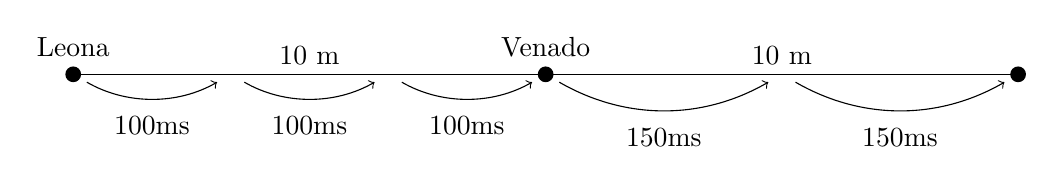
\begin{tikzpicture}[dot/.style={circle, minimum size=2mm, inner sep =0, fill, black}]
        \draw (0,0) node[dot, label=above:Leona] {} -- node[above] {10 m} (6,0) node[dot, label=above:Venado] {} -- node[above] {10 m} (12,0) node[dot] {};
        \foreach \i in {0,2,4}
            \draw[->, shorten >=2mm, shorten <=2mm] (\i,0) to [bend right] node[label=below:100ms]{} (\i+2,0);
        \foreach \i in {6,9}
            \draw[->, shorten >=2mm, shorten <=2mm] (\i,0) to [bend right] node[label=below:150ms]{} (\i+3,0);
    \end{tikzpicture}
    \end{center}

    Con el diagrama es fácil ver que la leona, para recorrer 10 metros, como da 3 pasos y en cada paso dura 100 milisegundos, va a durar en total 300 milisegundos. Y el venado da 2 pasos, durando en cada uno 150 milisegundos, es decir, para recorrer 10 metros dura 300 milisegundos. Es decir, ambos duran lo mismo en recorrer la misma distancia, por lo que tienen la misma velocidad. 

    Note entonces que cuando la leona llega donde estaba el venado originalmente, recorriendo 10 metros, el venado ya va a haber avanzado 10 metros en el mismo tiempo. Así, se mantienen siempre a la misma distancia de 10 metros. Por lo tanto, en 3000 milisegundos estarán a 10 metros de distancia. La respuesta correcta es la B.  \hfill $\square$

    {\small \itshape
    Otra opción es calcularlo todo. Como cada paso de la leona toma 100 ms, en 3000 ms da $3000/100 = 30$ pasos, y como cada 3 pasos son 10 metros, recorre $(30/3)\cdot 10 = 100$ metros en 3000 ms. De forma similar, el venado da $3000/150 = 20$ pasos en 3000 ms, de forma que como cada 2 pasos recorre 10 metros, en 20 pasos habrá recorrido 100 metros. Así, ambos recorren la misma longitud y por tanto se mantienen a la misma distancia original: 10 metros.}
\end{solution}

\question
Para un concurso se numeran consecutivamente los boletos empezando en 1. Si se han escrito 252 dígitos en total, ¿cuántos boletos se han numerado?
\begin{choices}
  \choice 118.
  \choice 119.
  \CorrectChoice 120.
  \choice 121.
\end{choices}

\begin{solution}
    En los primeros 9 boletos (1-9) se escribió un solo dígito. Nos quedan $252-9=243$ dígitos por escribir. Del 10 al 99, se escribieron dos dígitos pero, ¿cuántos números hay aquí? Si restamos $99-10$, no estamos contando el 10, por lo que la cantidad de números es $99-9=90$, es decir hay que restar el número anterior al primero que queremos contar. Si esto no les convence, intenten reflexionarlo hasta convencerse.

    Por lo tanto, del 10 al 99 escribimos $2\cdot90=180$ dígitos. Quedan por tanto $243-180=63$ dígitos. Como los siguientes números tienen 3 dígitos, faltan $63/3 = 21$ números de escribir. Como hasta ahora llegamos al 99 y faltan 21, el último número que se escribe es $99+21 = 120$. Por lo tanto, se numeraron (desde el 1 al 120), 120 boletos. La opción correcta es la C. \hfill $\square$
\end{solution}

\question
En una campaña de reciclaje, por cada botella reciclada se otorgan 150 puntos. Se requieren 400 puntos para reclamar un premio. Si el equipo de Ana obtuvo 3 premios, y quedó sin puntos, ¿cuántas botellas recicló?
\begin{choices}
  \choice 6.
  \choice 7.
  \choice 8.
  \choice 9.
\end{choices}

\begin{solution}
    En este caso lo más sencillo es hacer el problema en reversa. El equipo de Ana obtuvo 3 premios, cada uno cambiando 400 puntos, y quedaron sin puntos; por lo tanto, tenían $3\cdot400 = 1200$ puntos. Como cada botella reciclada otorga 150 puntos, para saber cuántas botellas reciclaron dividimos $1200/150$:
    \[
    \frac{1200}{150}=\frac{120}{15}=\frac{40\cdot\cancel3}{5\cdot\cancel3}=\frac{8\cdot5}{5}=8
    \]
    El equipo de Ana recició 8 botellas en total. La opción correcta es la C. \hfill $\square$
    
    {\small \itshape
    Otra posible solución es considerar cuántas botellas equivalen a un premio. Como cada botella son 150 puntos y cada premio son 400, ¿cuántas botellas necesitamos para hacer 400 puntos? $400/150 = 40/15 = 8/3$. Para obtener un premio, se necesitan ``$8/3$ de botella''. Por lo tanto, para tres premios se necesitan $(8/3) \cdot 3 = 8$ botellas.  }
\end{solution}

\question En una fábrica se empacó cierto producto de forma individual. La fábrica utilizó 2 máquinas para realizar este trabajo. La máquina antigua empacó 24 productos cada hora. La máquina nueva empacó 30 productos cada hora. Ayer la máquina antigua comenzó a empacar a las 7:00 a. m. y la máquina nueva comenzó a empacar a las 8:30 a. m.

¿Qué hora era cuando ambas máquinas llevaban la misma cantidad de producto empacado? \footnote{\cite{24preguntas}}

\begin{choices}
    \choice 9:30 a.m.
    \choice 11:30 a.m.
    \choice 2:30 p.m.
    \choice 3:30 p.m.
\end{choices}

Vamos a resolver el problema de tres formas distintas:

\begin{solution}
    Podemos hacerlo a fuerza bruta. Para esto podemos hacer un diagrama y visualizar cuántos productos ha empacado cada máquina a lo largo del tiempo. Note que una empieza a las 7:00 y otra a las 8:30, por lo que para compararlas, es mejor ir de media hora en media hora. Como en 1 hora las máquinas antigua y nueva empacan respectivamente 24 y 30 productos, en 30 minutos empacan 12 y 15 respectivamente. Hacemos la tabla:
    
    \begin{tabular}[t]{ccc}
        \begin{tabular}{c|c|c}
            Hora & Antigua & Nueva \\\hline
            7:00 & 0 & 0 \\
            7:30 & 12 & 0 \\
            8:00 & 24 & 0 \\
            8:30 & 36 & 0 \\
            9:00 & 48 & 15 \\
            9:30 & 60 & 30 \\
            10:00 & 72 & 45 \\
            10:30 & 84 & 60 \\
            11:00 & 96 & 75 \\
            11:30 & 108 & 90
        \end{tabular} &  & \begin{tabular}{c|c|c}
            Hora & Antigua & Nueva \\\hline
            12:00 & 120 & 105 \\
            12:30 & 132 & 120 \\
            1:00 & 144 & 135 \\
            1:30 & 156 & 150 \\
            2:00 & 168 & 165 \\\hline
            2:30 & 180 & 180 \\\hline
            3:00 & 192 & 195 \\
            3:30 & 204 & 210 \\
            &&\\
            &&
        \end{tabular}
    \end{tabular}

    Vemos entonces que a las 2:30 p.m. las máquinas llevaban la misma cantidad empacada, la C. es la respuesta correcta. \hfill $\square$
\end{solution}

    La segunda forma se relaciona con los problemas en que un depredador persigue una presa. En este caso la máquina nueva ``persigue a la nueva'':

\begin{solution}
    Hacemos el problema paso a paso
    \begin{enumerate}
        \item Cuando inicia la máquina nueva, ¿cuánto producto empacado lleva la antigua?: Ha pasado 1:30, por lo que la máquina antigua empacó 24 productos en una hora y 12 en la otra, para un total de 36 productos. 

        La máquina nueva debe cerrar la ``distancia'' de 36 productos, y puede hacerlo porque empaca más rápido.

        \item ¿por cuánto se reduce la diferencia de producto empacado? Veamos que mientras la vieja produce 24, la nueva produce 30. De esta forma, en una hora la máquina nueva reduce la ``distancia'' entre ella y la vieja en 6 productos.
        
        \item Como la máquina vieja inicia con 36 productos de ventaja, y cada hora se reduce esa diferencia en 6, es necesario que pasen $36/6=6$ horas desde que la nueva empezó a trabajar. Es decir, cuando pasen 6 horas, la máquina nueva habrá producido los 36 que le faltaban y ambas tendrán la misma cantidad de producto empacado.
    \end{enumerate}

    Como la nueva inició a las 8:30, tienen la misma cantidad de producto empacado a las $8\colon30 + 6\colon00 = 14\colon30 = 2\colon30 \text{ p.m.}$, la opción C.
    \hfill $\square$ \end{solution}

    Una tercera forma es resolviendo un sistema de ecuaciones, que veremos en el capítulo de álgebra.
    
\question
Una galaxia tiene dos planetas: P y Q. Cada
año del planeta P tiene 120 días terrestres. Por
otra parte, en el planeta Q, cada año tiene 140
días terrestres.

¿Qué cantidad de años en Q tiene un habitante
que tiene 7 años en P? \footnote{\cite{SEMA2021}}

\begin{choices}
    \choice 5
    \choice 6
    \choice 8
    \choice 9
\end{choices}

\begin{solution}
    Este es un problema de conversiones. Tenemos tres unidades: años en P, años en Q, y días terrestres, y tenemos conversiones de 1 año en P son 120 días terrestres, y 1 año en Q son 140 días terrestres. Luego, 7 años en P serían $120\cdot7 = 840$ días terrestres, y como cada 140 días de estos hacen 1 año en Q, dividimos esta cantidad entre 140: para hacerlo fácil, lo mejor es escribirlo como una fracción e ir cancelando factores comunes:
    \[
    \frac{840}{140} = \frac{84\!\cancel{0}}{14\!\cancel{0}} = \frac{\cancelto{42}{84}}{\cancelto{7}{14}} = \frac{42}{7} = 6 \text{ años de Q.}
    \]
    Lo que hicimos fue dividir primero entre 10 arriba y abajo, luego entre 2 y luego entre 7.

    Otra forma más rápida es no hacer el cálculo $120\cdot7$ días terrestres. Si lo dejamos así, y luego decimos que cada 140 días de estos es un año de Q, dividimos entre 140:
    \[
    \frac{120\cdot7}{140} = \frac{12\cdot\cancel{10}\cdot7}{14\cdot\cancel{10}} = \frac{6\cdot\cancel2\cdot \cancel7}{\cancel7\cdot \cancel2} = 6 \text{ años de Q.}
    \]
    Aquí cancelamos un 0 de arriba y abajo (sacando un 10 de 120 y uno de 140 y cancelándolos), luego cambiamos 12 por $6\cdot2$ y 14 por $7\cdot2$. Y cancelamos lo factores comunes del numerador y del denominador.

    \textbf{Forma alternativa:} Si no queremos dividir, la otra opción es pasar todo a días terrestres, incluyendo las opciones de respuesta. Sabemos que 7 años en P son 840 días terrestres, y luego las respuestas que nos dan son (usando que cada año en Q son 140 días terrestres):

    \begin{enumerate}[A.]
        \item 5 años en Q $= 5\cdot 140 = 10 \cdot70 = 700$ días terrestres (multipliqué el 5 por 2 y dividí el 140 entre 2 para hacer más fácil el cálculo).
        \item 6 años en Q $= 6 \cdot 140 = 600 + 240 = 840$ días terrestres (hice primero $6 \cdot 100$ y le sumé $6\cdot 40$).
        \item 8 años en Q $= 8 \cdot 140 = 800 + 320 = 1120$ días terrestres.
        \item 9 años en Q $= 9 \cdot 140 = 900 + 360 = 1260$ días terrestres.
    \end{enumerate}

    Así, comparando, debe ser la B. \hfill $\square$
\end{solution}




\question Carlos tenía 810 gapes en la billetera al inicio del día. Él decidió regalar la tercera parte del dinero que tuviera en la billetera a cada uno de los sobrinos que llegara a su casa ese día.

¿Cuánto dinero le dio Carlos al tercer sobrino que lo visitó?
\begin{choices}
    \choice 81 gapes
    \choice 270 gapes
    \choice 90 gapes
    \CorrectChoice 120 gapes %%%%%%
    \choice 30 gapes
\end{choices}

\question Los asientos de un carrusel están numerados con 1, 2, 3, y así sucesivamente de forma consecutiva y circular. Un niño está sentado en el número 11 y otro está sentado en el número 4, que está diametralmente opuesto. Entonces, la cantidad de asientos que tiene el carrusel es\footnote{\cite{OLCOMAN1-2021}}
\begin{choices}
    \choice 13
    \choice 14
    \choice 16
    \choice 17
\end{choices}
    
\end{questions}

\subsection{Operaciones con fracciones}

\begin{questions}
    \question Resuelva y simplifique al máximo los siguientes productos y divisiones de fracciones. Sugerencia: Simplifique antes de hacer las operaciones, cancelando factores en común de los números en el numerador con aquellos en el denominador.

    \begin{multicols}{3}
        \begin{parts}
            \part $\dfrac{23}{15}\cdot\dfrac{10}{12} =$
            \part $\dfrac{81}{49}\cdot\dfrac{7}{45} =$
            \part $\dfrac{10}{56}\cdot\dfrac{21}{320}$
            \part $\dfrac{9	}{2	}\cdot\dfrac{ 5}{12}$
            \part $\dfrac{64}{60}\cdot\dfrac{30}{8 }$
            \part $\dfrac{23}{27}\cdot\dfrac{90}{46}$
            \part $\dfrac{45}{78}\cdot\dfrac{42}{30}$
            \part $\dfrac{72}{84}\cdot\dfrac{175}{50}$
            \part $\dfrac{91}{99}\cdot\dfrac{55}{13}$
            \part $\dfrac{14}{9}\cdot\dfrac{21}{2}$
            \part $\dfrac{30}{19}\cdot\dfrac{19}{550}$
            \part $\dfrac{35}{36}\cdot\dfrac{84}{85}$
            \part $\dfrac{41}{64}\cdot\dfrac{86}{82}$
            \part $\dfrac{11}{95}\cdot\dfrac{85}{22}$
            \part $\dfrac{64}{44}\cdot\dfrac{121}{54}$
            % \part $\dfrac{85}{19}\cdot\dfrac{93}{25}$
            % \part $\dfrac{35}{28}\cdot\dfrac{84}{89}$
            % \part $\dfrac{29}{39}\cdot\dfrac{72}{67}$
            % \part $\dfrac{75}{88}\cdot\dfrac{26}{48}$
            % \part $\dfrac{44}{90}\cdot\dfrac{53}{97}$
            % \part $\dfrac{72}{53}\cdot\dfrac{28}{51}$
            % \part $\dfrac{62}{62}\cdot\dfrac{38}{55}$
            % \part $\dfrac{89}{69}\cdot\dfrac{89}{39}$
            % \part $\dfrac{43}{83}\cdot\dfrac{48}{16}$
            % \part $\dfrac{79}{71}\cdot\dfrac{65}{99}$
            % \part $\dfrac{46}{69}\cdot\dfrac{72}{93}$
            % \part $\dfrac{70}{30}\cdot\dfrac{96}{64}$
            % \part $\dfrac{38}{17}\cdot\dfrac{24}{74}$
            % \part $\dfrac{36}{86}\cdot\dfrac{79}{45}$
            % \part $\dfrac{33}{67}\cdot\dfrac{19}{66}$
            % \part $\dfrac{66}{97}\cdot\dfrac{91}{93}$
            % \part $\dfrac{50}{39}\cdot\dfrac{29}{89}$
            % \part $\dfrac{52}{27}\cdot\dfrac{32}{73}$
            % \part $\dfrac{18}{86}\cdot\dfrac{59}{58}$
            % \part $\dfrac{27}{45}\cdot\dfrac{57}{52}$
            % \part $\dfrac{78}{61}\cdot\dfrac{98}{19}$
            % \part $\dfrac{31}{88}\cdot\dfrac{39}{35}$
            % \part $\dfrac{46}{17}\cdot\dfrac{60}{52}$
            % \part $\dfrac{39}{72}\cdot\dfrac{92}{49}$
            % \part $\dfrac{24}{57}\cdot\dfrac{46}{57}$
            % \part $\dfrac{37}{88}\cdot\dfrac{39}{35}$
            % \part $\dfrac{76}{13}\cdot\dfrac{94}{88}$
        \end{parts}
    \end{multicols}

    \question El resultado de la operación 
    \[
    \left[\left(\frac{7}{12}+\frac{3}{16}\right)-\left(\frac{9}{32}-\frac{7}{40}\right)\right]\div\left(1-\frac{13}{16}\right)
    \]
    es\footnote{\cite{OLCOMAN1-2021}}
    \begin{choices}
        \choice $\dfrac{319}{30}$
        \choice $\dfrac{319}{90}$
        \choice $\dfrac{421}{90}$
        \choice $\dfrac{421}{30}$
    \end{choices}

    \question Si $a=2$ y $b=3$, la expresión
    \[
    \frac{\dfrac{a}{b} + \dfrac{b}{a}}{\dfrac{b}{a}+\dfrac{1}{ab}}-1
    \]
    es equivalente a\footnote{\cite{OLCOMAN1-2021}}

    \begin{choices}
        \choice $\dfrac{23}{10}$
        \choice $\dfrac{1}{2}$
        \choice $\dfrac{3}{10}$
        \choice $-\dfrac{3}{2}$
    \end{choices}
\end{questions}

\subsection{Problemas con números racionales}
\begin{questions}

\question
David tiene dos calculadoras $P$ y $Q$. La calculadora $P$ resuelve las operaciones normalmente. La calculadora $Q$ cambia los números de una operación por el doble de estos. Así, por ejemplo, cuando se ingresa la operación $3\cdot6$, se calcula la operación $6 \cdot 12$. David realiza operaciones básicas en ambas calculadoras y se da cuenta que hay una operación que al aplicarla a una pareja de números, en cualquiera de las calculadoras, $P$ o $Q$, el resultado es el mismo.

¿Cuál es, con certeza, la operación en la que David obtiene el mismo resultado? \footnote{\cite{practicaUCR1}}

\begin{choices}
    \choice Suma.
    \choice Resta.
    \choice División.
    \choice Multiplicación.
\end{choices}

\begin{solution}
    Podemos hacer casos tomando un ejemplo muy básico, como 2 y 1. 
    \begin{enumerate}[A.]
        \item En la calculadora $P$, $2+_{_P}1 = 2+1 = 3$. En la calculadora $Q$, $2+_{_Q}1 = 4+2 = 6$. Como $3\neq 6$, no puede ser suma.
        \item En la calculadora $P$, $2-_{_P}1 = 2-1=1$. En la $Q$, $2-_{_Q}1 = 4-2 = 2$, que son distintos. Así, no es la resta.
        \item En $P$, $2\div_{_P}1 = \frac{2}{1} = 2$, y en $Q$, $2\div_{_Q}1 = \frac{4}{2}=2$. La división podría funcionar. No podemos estar seguros aún pues solo es un ejemplo, un caso muy particular.
        \item En $P$, $2\cdot_{_P}1 = 2\cdot1 = 2$, en $Q$, $2\cdot_{_Q}1 = 4\cdot2 = 8$. Son distintos, luego la multiplicación no es.
    \end{enumerate}
    Por descarte, la opción correcta es la C.

    En general es cierto, pues si $a, b$ son dos números, $a\div_{Q}b = \frac{2a}{2b} = \frac{a}{b} = a\div b = a\div_{_P}b$, pues podemos cancelar el 2 de arriba y abajo. \hfill $\square$
\end{solution}

\question
Camila tiene un frasco completamente lleno de miel. Ella quiere vaciar toda la miel en 4 recipientes pequeños.

Según esta información, ¿cuál de las siguientes opciones es imposible que suceda? \footnote{\cite{60-10preguntas}}

\begin{choices}
    \choice Los cuatro recipientes quedarían con la misma cantidad de miel.
    \choice Dos recipientes quedarían con la misma cantidad de miel y los otros dos con cantidades distintas.
    \CorrectChoice Dos recipientes quedarían cada uno con una sexta parte de la miel, uno con la mitad y otro con la tercera parte.
    \choice Dos recipientes quedarían cada uno con una tercera parte y los otros dos con una sexta parte cada uno.
\end{choices}

\question
María fue de compras el sábado, se gastó la tercera parte de lo que llevaba en un par de tenis, la cuarta parte del resto en un abrigo. Al final del día, quiere comprar un bolso cuyo precio es igual a cinco doceavos de lo que llevaba por la mañana.

Entonces se puede asegurar con certeza que María\footnote{\cite{SEMA2022}}
\begin{choices}
    \choice no tiene suficiente dinero para comprar el bolso.
    \choice compra el bolso y no le sobra nada.
    \choice compra el bolso y le sobra un doceavo de lo que llevaba.
    \choice puede comprar dos bolsos iguales.
\end{choices}

\question
Lucía tiene cuatro sobrinos Alejandra, Lucía, Mario y José, decide repartir sus ahorros entre ellos de manera que a Alejandra le dio la cuarta parte, a Lucía la tercera parte del resto, a Mario la mitad de lo que quedaba y a José lo que quedó. Entonces con certeza sucederá que\footnote{\cite{SEMA2022}}
\begin{choices}
    \choice todos recibieron la misma cantidad de dinero.
    \choice Alejandra recibió menos dinero que Mario.
    \choice José recibió más dinero que Lucía.
    \choice José recibió más dinero que Mario.
\end{choices}

\question
Pedro tiene un tanque lleno de agua y desea repartirla entre varios baldes.

Primero llena $\dfrac{1}{4}$ del tanque en un balde grande. Luego reparte la mitad de lo que queda en dos baldes medianos, en partes iguales. Finalmente, llena un último balde con el resto del agua.

¿Cuál de las siguientes afirmaciones es verdadera?

\begin{choices}
    \choice El último balde contiene la misma cantidad que el balde grande.
    \choice Cada balde mediano contiene más que el balde grande.
    \choice El último balde contiene menos que cualquier otro balde.
    \choice El agua del tanque se distribuye en partes exactamente iguales entre los cuatro baldes.
\end{choices}

\question
Isabel horneó un pastel para compartirlo con sus amigas. Primero le dio a Ana la quinta parte del pastel. Luego, le dio a Beatriz la tercera parte de lo que quedaba. Después, le dio a Carmen la mitad de lo que aún quedaba y se quedó con lo restante.

¿Cuál fracción del pastel se quedó Isabel?

\begin{choices}
    \choice $\dfrac{1}{5}$
    \choice $\dfrac{4}{15}$
    \choice $\dfrac{7}{30}$
    \choice $\dfrac{1}{3}$
\end{choices}

\question
Julián recorrió un sendero de montaña. En la primera hora caminó un tercio del camino. En la segunda hora recorrió la mitad de lo que le faltaba. En la tercera hora caminó la mitad de lo que aún faltaba después de la segunda hora.

¿Qué parte del camino le falta por recorrer después de la tercera hora?

\begin{choices}
    \choice $\dfrac{1}{6}$
    \choice $\dfrac{1}{8}$
    \choice $\dfrac{1}{12}$
    \choice $\dfrac{1}{4}$
\end{choices}

\end{questions}

\printnotes